\section{Resultados}\label{sec:resultados}

Os resultados a seguir avaliam a instanciação descrita na Seção \ref{sec:metodologia}, e não o método em si, cujas propriedades (semidefinição positiva, pseudométrica e decomposição da energia espectral) foram demonstradas nas Seções \ref{sec:tensor_rkhs} a \ref{sec:representation_geometry}. Eles são apresentados na ordem das perguntas da Subseção \ref{subsec:perguntas}, e, salvo menção explícita, os valores são os da variante de \textbf{alvo fixo}. O motivo dessa convenção fica claro com um exemplo. Na ResNet, os $k$ vizinhos mais próximos de uma imagem na Gram conjunta de \texttt{b3} recuperam a predição do modelo em $95{,}6\%$ dos casos quando o gradiente é tomado em relação à classe predita, e em apenas $20{,}4\%$ com alvo fixo. A primeira leitura não é um acerto do método: o gradiente já carrega a predição, e reencontrá-la é como procurar uma resposta que foi escrita na pergunta.

\subsection{P1: A geometria reflete o comportamento do modelo?}\label{subsec:res_comportamento}

Se o espaço reflete o entendimento do modelo, os vizinhos de uma amostra devem ter a mesma predição que ela, as amostras que o modelo erra devem estar em regiões ambíguas e as classes que o modelo confunde devem estar próximas entre si. A Tabela \ref{tab:res_estabilidade} e a Figura \ref{fig:res_estabilidade} apresentam essas leituras para as dez bases tabulares.

\begin{table}[htbp]
\centering
\caption{Leituras de comportamento nas dez bases tabulares (cinquenta execuções, alvo fixo). Média entre bases, do \texttt{stem} a \texttt{b6}, o piso cruzado da Gram conjunta, que é plano na profundidade, e a fração das execuções em que a Gram conjunta supera estritamente esse piso. As leituras espectrais não se aplicam à análise representacional (RSA).}
\label{tab:res_estabilidade}
\footnotesize
\setlength{\tabcolsep}{4pt}
\begin{tabular}{l c c c c c}
\hline
Leitura & Conjunta & Ativações & RSA & Piso & Acima do piso \\
\hline
$k$-vizinhos contra a predição & $0{,}882 \to 0{,}975$ & $0{,}851 \to 0{,}974$ & $0{,}852 \to 0{,}974$ & $0{,}805$ & 100\% \\
AUC da margem para o acerto & $0{,}824 \to 0{,}965$ & $0{,}804 \to 0{,}961$ & $0{,}764 \to 0{,}940$ & $0{,}767$ & 81\% a 100\% \\
Confusão suave (Spearman) & $0{,}463 \to 0{,}400$ & $0{,}460 \to 0{,}447$ & $0{,}354 \to 0{,}342$ & $0{,}422$ & 44\% a 76\% \\
Contenção em $V_r$ ($r = K-1$) & $0{,}568 \to 0{,}831$ & $0{,}475 \to 0{,}826$ & & $0{,}416$ & 100\% \\
$\widehat{E}_{\mathrm{ratio}}$ para o erro & $0{,}658 \to 0{,}788$ & $0{,}635 \to 0{,}787$ & & $0{,}598$ & 84\% a 100\% \\
\hline
\end{tabular}
\end{table}

\begin{figure}[htbp]
    \centering
    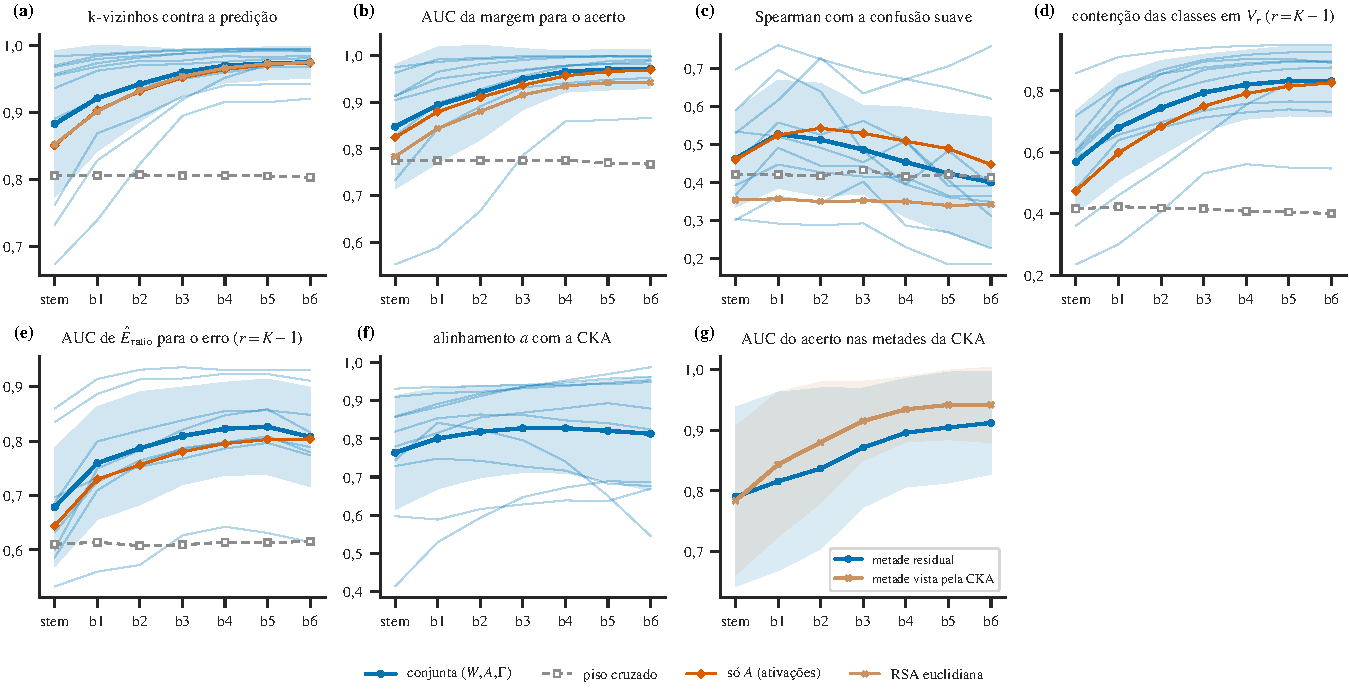
\includegraphics[width=\textwidth]{figuras/res_estabilidade.pdf}
    \caption{Leituras por bloco nas dez bases tabulares, com alvo fixo. A linha grossa é a média entre bases da Gram conjunta, as linhas finas são as bases isoladas e a faixa é o desvio entre bases. A linha tracejada é o piso cruzado, e as demais séries são a fonte de ativações isolada e a análise representacional euclidiana. (a) Recuperação da predição por $k$-vizinhos. (b) Área sob a curva ROC da margem geométrica para o acerto. (c) Concordância com a confusão suave. (d) Contenção das direções de classe em $V_r$. (e) $\widehat{E}_{\mathrm{ratio}}$ como preditor do erro. (f) Alinhamento com a Gram das ativações. (g) Acerto previsto pelas duas partes da decomposição contra a CKA.}
    \label{fig:res_estabilidade}
\end{figure}

A recuperação da predição por $k$-vizinhos fica acima do piso em todas as execuções e em todos os blocos (Figura \ref{fig:res_estabilidade}a). O piso, entretanto, é alto ($0{,}805$), e isso é uma propriedade dos dados: as classes dessas bases já são quase separáveis nos atributos brutos, e um modelo na inicialização preserva boa parte dessa estrutura. Por esse motivo, o Oxford-IIIT Pet funciona como contraprova. Com 37 raças, o piso cai para cerca de $0{,}06$, e a Gram conjunta da ResNet cresce de $0{,}069$ no \texttt{stem} para $0{,}603$ em \texttt{b6}, acima do piso em todas as sementes a partir de \texttt{b1} (Figura \ref{fig:res_pets}a).

A segunda leitura é a mais diretamente útil. A margem geométrica de uma amostra, isto é, o quanto ela está mais próxima de amostras com a sua própria predição do que de amostras com outras predições, prevê se o modelo a acerta, acima do piso nas bases tabulares e em todas as sementes e blocos do Pet (Figuras \ref{fig:res_estabilidade}b e \ref{fig:res_pets}b). A intuição é a mesma do \textit{trust score} \citep{Jiang2018} e dos $k$-vizinhos profundos \citep{Papernot2018}: uma predição cercada de vizinhos classificados de outra forma merece menos confiança. Na prática, essa leitura permite encaminhar as predições menos plausíveis de um modelo implantado para revisão humana. Ela ainda não foi comparada à confiança do próprio \textit{softmax} \citep{Hendrycks2017}.

A terceira leitura, a concordância com a confusão, separa as duas famílias de dados. Nas bases tabulares, ela não se sustenta nos blocos profundos, ficando acima do piso em apenas 44\% a 47\% das execuções em \texttt{b5} e \texttt{b6} (Figura \ref{fig:res_estabilidade}c). No Pet, ela cresce de $0{,}170$ para $0{,}674$, contra um piso em torno de $0{,}21$, e supera o piso em todas as sementes a partir de \texttt{b1} (Figura \ref{fig:res_pets}c). A diferença é simples: nas bases tabulares o modelo quase não erra, e a confusão entre a maior parte dos pares de classes é praticamente nula. No Pet, raças confundíveis produzem uma estrutura de confusão rica, e a geometria a reproduz.

\begin{figure}[htbp]
    \centering
    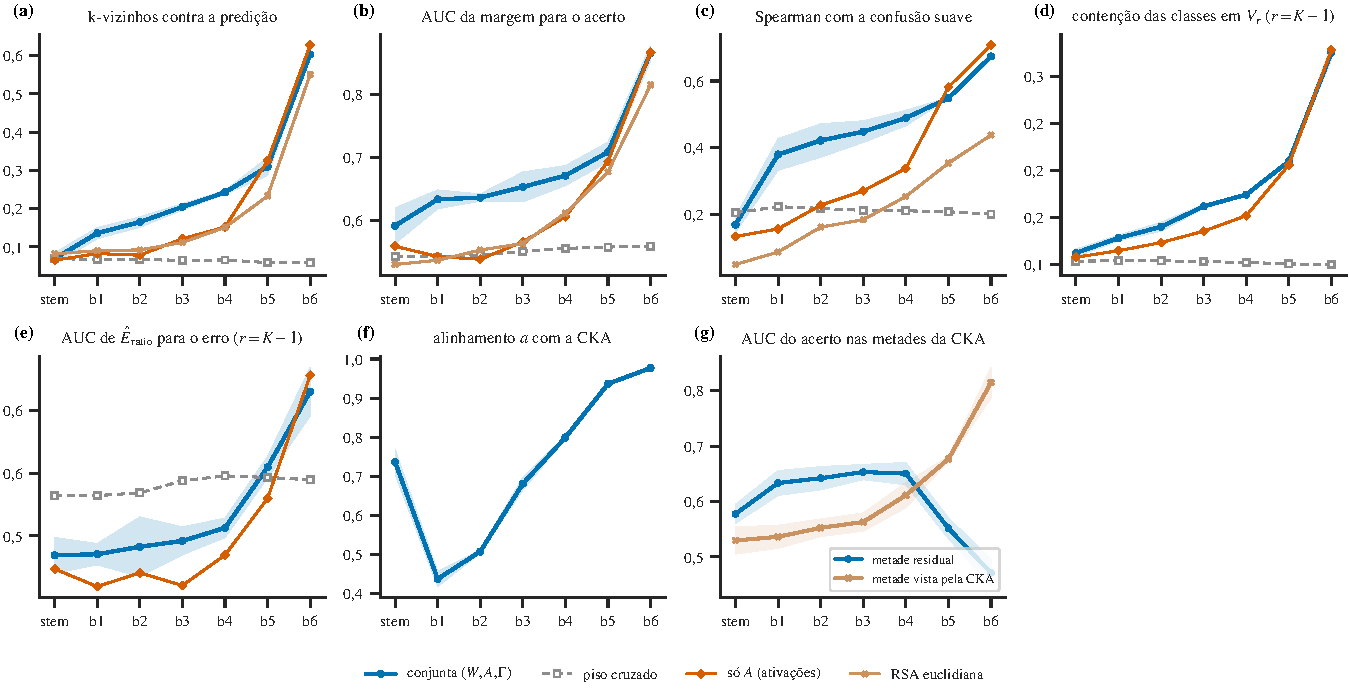
\includegraphics[width=\textwidth]{figuras/res_pets.pdf}
    \caption{As mesmas leituras da Figura \ref{fig:res_estabilidade} no Oxford-IIIT Pet, com a ResNet (três sementes, alvo fixo). A faixa é o desvio entre sementes. Diferentemente das bases tabulares, o piso do $k$-vizinhos fica próximo do acaso ($1/37$), e a concordância com a confusão supera o piso a partir de \texttt{b1}.}
    \label{fig:res_pets}
\end{figure}

A resposta a P1 é, portanto, afirmativa para a decisão e para o erro, e condicionada para a confusão, que só se sustenta quando o modelo confunde classes de forma estruturada.

\subsection{P2: A composição acrescenta algo às fontes isoladas?}\label{subsec:res_composicao}

A resposta depende de onde a leitura é feita. Nas bases tabulares, a Gram conjunta supera a fonte de ativações na recuperação da predição em 90\% das execuções no \texttt{stem}, mas essa vantagem decresce até 32\% em \texttt{b6}. No Pet, o padrão é o mesmo e mais nítido: a conjunta supera as ativações em todas as sementes de \texttt{b1} a \texttt{b4}, nas três leituras de comportamento, e a vantagem desaparece nos dois últimos blocos (Figura \ref{fig:res_pets}). Contra a RSA, a composição vence na previsão do acerto em 84\% a 91\% das execuções tabulares e em todas as sementes e blocos da ResNet.

A origem da vantagem é o gradiente contrastivo. Nos blocos rasos, as ativações descrevem o conteúdo local da imagem (bordas, texturas e cores), e duas imagens de raças diferentes com o mesmo fundo parecem semelhantes para $A$. O gradiente, por outro lado, descreve como a decisão responderia a uma mudança naquele estado, e já é específico da classificação. De fato, na ResNet, $\Gamma$ isolado praticamente iguala a composição de \texttt{b1} a \texttt{b4}. Nos blocos profundos, as ativações já carregam a decisão, e a composição deixa de acrescentar.

\subsection{P3: O método se distingue de uma simples CKA?}\label{subsec:res_cka}

A decomposição $\hat{\mathbf{G}} = a\,\hat{K}_{\mathrm{ativ}} + R$ responde a essa pergunta em termos de conteúdo. Um resultado torna a decomposição fácil de interpretar: a parte vista pela CKA, $a\,\hat{K}_{\mathrm{ativ}}$, produz exatamente os mesmos valores que a RSA euclidiana em todas as leituras, sementes e arquiteturas. Isso não é coincidência, visto que as distâncias induzidas pela Gram linear centrada das ativações são as distâncias euclidianas entre elas. A parte que a CKA enxerga é, portanto, a geometria euclidiana das ativações, e o resíduo $R$ é tudo aquilo que uma análise das ativações não enxerga.

Nas bases tabulares, o alinhamento $a$ fica entre $0{,}76$ e $0{,}83$, e o resíduo prevê o acerto pior do que a parte vista em cerca de três quartos das execuções (Figura \ref{fig:res_estabilidade}g), o que favorece a CKA. Na ResNet, o resultado se inverte nos blocos rasos e intermediários: o alinhamento cai para $0{,}44$ em \texttt{b1}, e o resíduo prevê o acerto melhor do que a parte vista em todas as sementes do \texttt{stem} a \texttt{b4}, invertendo-se nos dois últimos blocos, onde o alinhamento sobe para $0{,}94$ e $0{,}98$ (Figura \ref{fig:res_pets}, painéis f e g). A resposta a P3 é, portanto, condicionada da mesma forma que P2: o método vê algo além da CKA onde as ativações ainda não carregam a decisão. Esse resultado é coerente com as limitações da CKA apontadas pela literatura, que mostram que ela é dominada pelos modos de maior variância das ativações \citep{Davari2023, Klabunde2025}.

\subsection{P4: A energia espectral descreve como o modelo representa cada amostra?}\label{subsec:res_espectro}

As leituras espectrais decompõem a Gram em modos e perguntam quais direções concentram a estrutura do espaço e quanto de cada amostra vive fora delas. A primeira afirmação, de que as direções de classe estão contidas em $V_r$, é a mais robusta da instanciação. Com $r = K-1$, ela supera o piso em todas as execuções tabulares e em todos os blocos, e a Gram conjunta supera as ativações em 88\% a 100\% das execuções em toda a profundidade (Figura \ref{fig:res_estabilidade}d). No Pet, os valores são menores, de $0{,}112$ para $0{,}325$, mas ficam acima do piso de $0{,}10$ a partir de \texttt{b1} (Figura \ref{fig:res_pets}d). Isto é, as poucas direções dominantes do espaço construído são as direções em que o modelo separa as suas decisões, e a composição concentra essa separação em menos modos do que as ativações.

A segunda afirmação depende da base. Nas bases tabulares, $\widehat{E}_{\mathrm{ratio}}$ prevê o erro acima do piso em 84\% a 100\% das execuções (Figura \ref{fig:res_estabilidade}e). Na ResNet, por outro lado, ela fica abaixo do piso do \texttt{stem} a \texttt{b4} e só o supera nos dois últimos blocos (Figura \ref{fig:res_pets}e). A ideia é a mesma da detecção de amostras fora da distribuição pelo resíduo do subespaço principal \citep{Wang2022ViM}, e o resultado mostra que esse indício só é confiável onde $V_r$ já é o subespaço da decisão. A razão de energia ortogonal é, portanto, a leitura menos robusta da instanciação.

\subsection{P5: O campo de energia e os conjuntos de nível apontam o que o modelo utiliza na entrada?}\label{subsec:res_campo}

Esta subseção toma como objetos as posições espaciais de uma única imagem, conforme o Comentário \ref{rem:diagnostic}. Em cada bloco, a posição $s$ carrega as três fontes, e as matrizes de Gram de ordem $P = HW$ são compostas pelo produto de Hadamard sem a normalização angular, que fixaria a energia de todas as posições. O campo de energia é a energia retida $\widehat{E}_{s,\parallel}$ da Equação \eqref{eq:empirical_energies}, calculada sobre 111 imagens de teste. A utilidade dessa leitura é auditar \textit{onde} o modelo olha, visto que um modelo pode acertar apoiando-se no fundo ou em um artefato da coleta \citep{Geirhos2020}.

\begin{figure}[htbp]
    \centering
    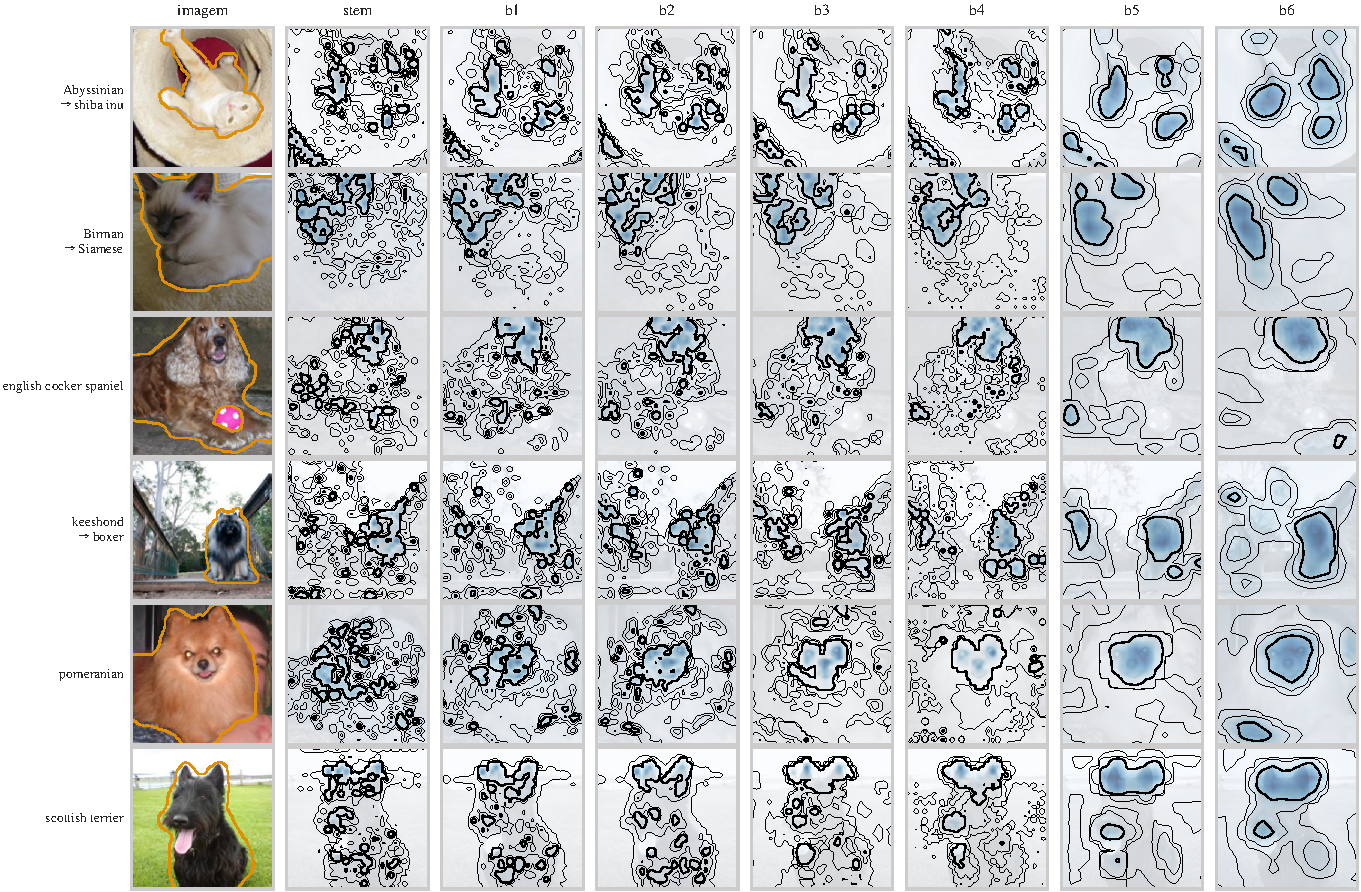
\includegraphics[width=\textwidth]{figuras/res_campo_resnet.pdf}
    \caption{Campo de energia da Gram conjunta da ResNet sobre seis imagens de teste do Oxford-IIIT Pet, do \texttt{stem} a \texttt{b6}. O contorno laranja na primeira coluna é a máscara do animal, utilizada apenas na avaliação, e os rótulos indicam a raça verdadeira e, quando o modelo erra, a predita. Tons escuros indicam maior energia retida.}
    \label{fig:res_campo_resnet}
\end{figure}

A primeira parte da pergunta é respondida afirmativamente. Na ResNet, o campo concentra de $0{,}82$ a $0{,}90$ da sua energia sobre o animal, contra $0{,}50$ de acaso, $0{,}66$ de um mapa que marca apenas o centro, $0{,}53$ a $0{,}78$ do Grad-CAM \citep{Selvaraju2017} e $0{,}47$ a $0{,}49$ da rede não treinada. Nos blocos rasos, o campo se espalha sobre o contorno e a textura do animal, e nos profundos se concentra em poucas regiões, tipicamente a cabeça (Figura \ref{fig:res_campo_resnet}). O campo também passa na verificação por aleatorização dos pesos \citep{Adebayo2018}, com correlação entre os campos da rede treinada e da não treinada próxima de zero.

A segunda parte não se sustenta com a mesma força. No teste de deleção \citep{Samek2017, Tomsett2020}, a Gram conjunta obtém de $0{,}47$ a $0{,}54$, contra $0{,}37$ do centro, e o Grad-CAM, calculado sobre o mesmo estado e o mesmo gradiente, a supera a partir de \texttt{b4}. Isto é, localizar o objeto e identificar a evidência da decisão são tarefas diferentes: um mapa pode cobrir todo o animal e, ainda assim, ordenar mal as suas partes \citep{Hooker2019, Nauta2023}.

\begin{figure}[htbp]
    \centering
    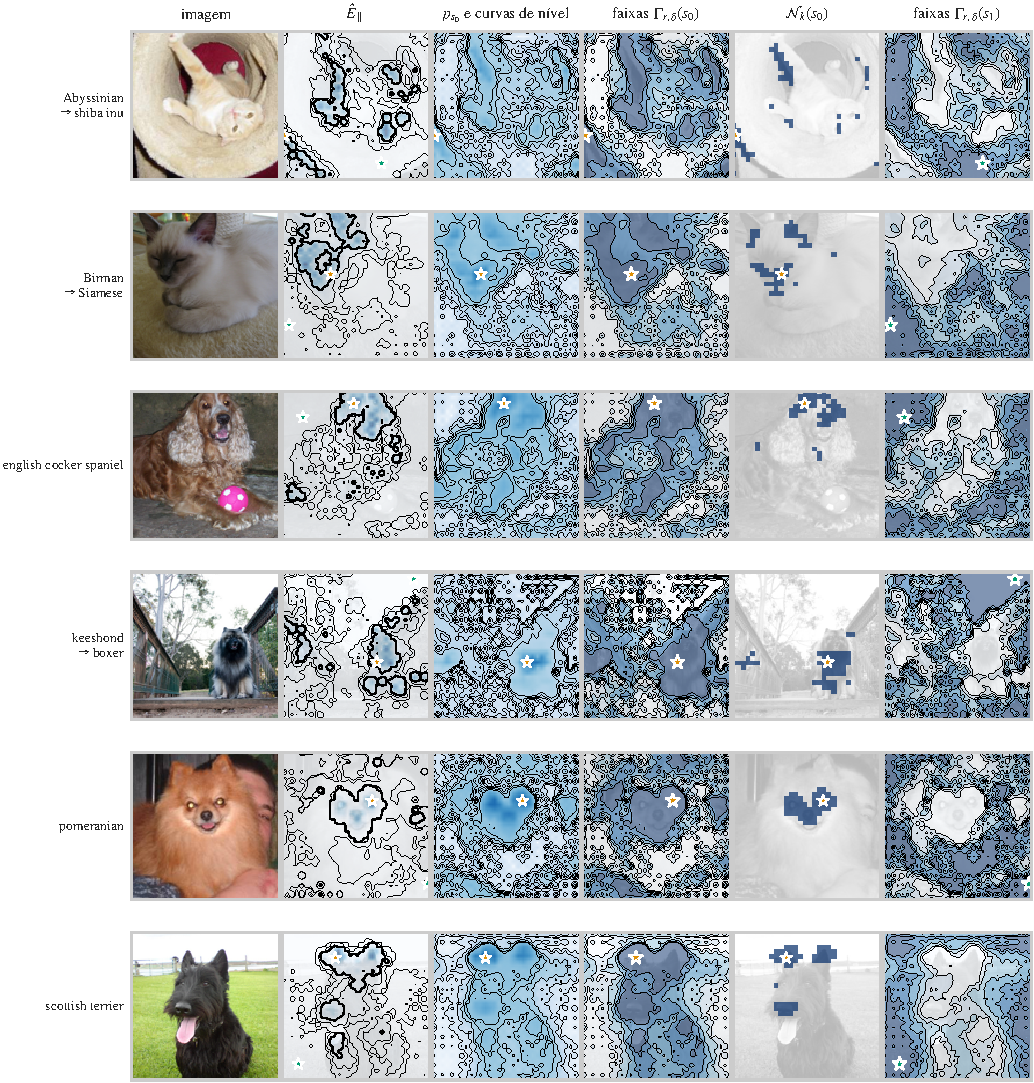
\includegraphics[width=\textwidth]{figuras/res_niveis.pdf}
    \caption{Conjuntos de nível no bloco \texttt{b4} da ResNet. Da esquerda para a direita, a figura mostra a imagem, o campo de energia com a referência $s_0$ (estrela laranja, medoide das posições de maior energia) e $s_1$ (estrela verde, medoide da metade de menor energia), a função distância $p_{s_0}$ com as suas curvas de nível, as faixas de nível $\Gamma_{r,\delta}(s_0)$, a vizinhança $\mathcal{N}_k(s_0)$ e as faixas em torno de $s_1$. No primeiro exemplo, $s_0$ cai na borda da imagem, sobre a faixa de energia alta produzida pelo preenchimento com zeros das convoluções.}
    \label{fig:res_niveis}
\end{figure}

Os conjuntos de nível da Equação \eqref{eq:sample_level_band} respondem à terceira parte: a partir de uma posição de referência $s_0$, quais regiões o modelo representa de forma semelhante? Para que a distância meça padrão, e não intensidade, a matriz do campo recebe a transformação angular $T_a$, e $s_0$ é o medoide das posições de maior energia. Com essa construção, a vizinhança de $s_0$ cai sobre o animal em $0{,}66$ no \texttt{stem} e em $0{,}90$ a $0{,}93$ nos blocos profundos, contra $0{,}44$ a $0{,}49$ da rede não treinada. A Figura \ref{fig:res_niveis} mostra o que essa leitura acrescenta ao campo: a vizinhança de $s_0$ reúne as regiões da cabeça, e não o corpo inteiro, isto é, separa as partes do animal que o modelo representa da mesma forma. Apagar as regiões na ordem da distância a $s_0$ remove a margem do modelo com diferença de áreas de $0{,}57$ a $0{,}59$ em \texttt{b4} e \texttt{b5}, contra no máximo $0{,}17$ da rede não treinada. Como mostra o primeiro exemplo da figura, a seleção de $s_0$ deve excluir a borda da imagem.

\subsection{P6: Por que esta amostra foi classificada de forma diferente daquela?}\label{subsec:res_diferencas}

Esta é a forma local do método e a mais próxima da maneira como as pessoas pedem explicações, que é contrastiva: não se pergunta por que algo aconteceu, e sim por que aconteceu isto em vez daquilo \citep{Miller2019}. Para cada amostra $i$, o par $j$ é o seu contrafactual observado mais próximo, e o método ordena as diferenças entre as duas pela pontuação $\Delta d_f$ da Equação \eqref{eq:delta_d}. A validação constrói contrafactuais sintéticos: se os primeiros atributos do ranking forem de fato os que distinguem as duas amostras para o modelo, levá-los ao valor de $j$ deve mudar a predição de $i$ para a de $j$ com poucas trocas.

\subsubsection*{Nas dez bases tabulares}

Sobre as dez bases e três sementes, com cinquenta pares por execução, a área sob a curva de trocas do método em \texttt{b3} é de $0{,}810$, contra $0{,}384$ da ordem aleatória e $0{,}607$ da rede não treinada, e o método supera essas duas referências em todas as execuções (Figura \ref{fig:res_diferencas}). Ele vence a atribuição de primeira ordem $\nabla f \cdot \Delta x$ em 87\% das execuções, mas empata com a diferença bruta $|\Delta x|$ ($0{,}812$), vencendo em 57\%. A área do método cresce com a profundidade do bloco, enquanto a da rede não treinada permanece plana, o que é coerente com P2: quanto mais a representação organiza a decisão, mais a distância nela aponta o que decide.

\begin{figure}[htbp]
    \centering
    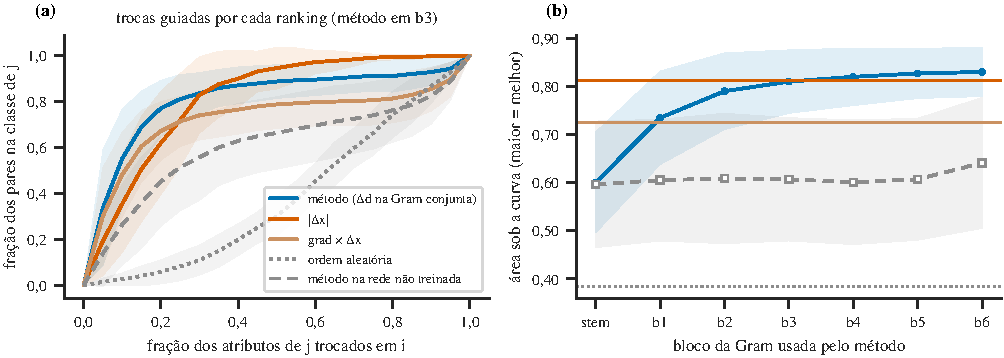
\includegraphics[width=\textwidth]{figuras/res_diferencas.pdf}
    \caption{Diferenças entre amostras nas dez bases tabulares. (a) Fração dos pares em que a amostra $i$ passa a ser classificada como $j$ conforme os $k$ primeiros atributos de cada ranking são trocados. (b) Área sob essa curva em função do bloco cuja Gram conjunta define o ranking, com as referências e o piso da rede não treinada.}
    \label{fig:res_diferencas}
\end{figure}

\subsubsection*{Estudo de caso: o método, o SHAP, o LIME e uma árvore de decisão}

Na \texttt{letter}, o perceptron atinge acurácia de $0{,}973 \pm 0{,}002$, e cada amostra difere do seu contrafactual, em média, em $9{,}4$ dos 16 atributos. A Tabela \ref{tab:res_letter} e a Figura \ref{fig:res_letter} reúnem os resultados sobre quinhentos pares.

\begin{table}[htbp]
\centering
\caption{Estudo de caso na \texttt{letter} (cinco sementes, cem pares por semente). Teste contrafactual de trocas (área sob a curva) e posição, em cada ranking, do atributo em que uma árvore de decisão treinada sobre os rótulos separa $i$ de $j$, nos pares em que ela reproduz as duas predições do perceptron (cerca de 71 por semente).}
\label{tab:res_letter}
\small
\begin{tabular}{l c c c}
\hline
Ranking & Área de trocas & Corte da árvore em 1º & Entre os 3 primeiros \\
\hline
Shapley exato com $j$ de referência & $0{,}862$ & $0{,}447$ & $0{,}737$ \\
\textbf{Método} (Gram conjunta, \texttt{b3}) & $\mathbf{0{,}803}$ & $\mathbf{0{,}416}$ & $\mathbf{0{,}691}$ \\
SHAP, $\phi(x_j) - \phi(x_i)$ & $0{,}775$ & $0{,}317$ & $0{,}657$ \\
LIME contrastivo, margem $f_{c_j} - f_{c_i}$ & $0{,}774$ & $0{,}388$ & $0{,}678$ \\
$|\Delta x|$ & $0{,}766$ & $0{,}262$ & $0{,}598$ \\
$\nabla f \cdot \Delta x$ & $0{,}711$ & $0{,}363$ & $0{,}572$ \\
SHAP só da amostra $i$ & $0{,}652$ & $0{,}233$ & $0{,}495$ \\
LIME só da amostra $i$ & $0{,}565$ & $0{,}218$ & $0{,}412$ \\
Método na rede não treinada & $0{,}651$ & $0{,}254$ & $0{,}510$ \\
Aleatória entre os que diferem & $0{,}639$ & $0{,}090$ & $0{,}316$ \\
\hline
\end{tabular}
\end{table}

\begin{figure}[htbp]
    \centering
    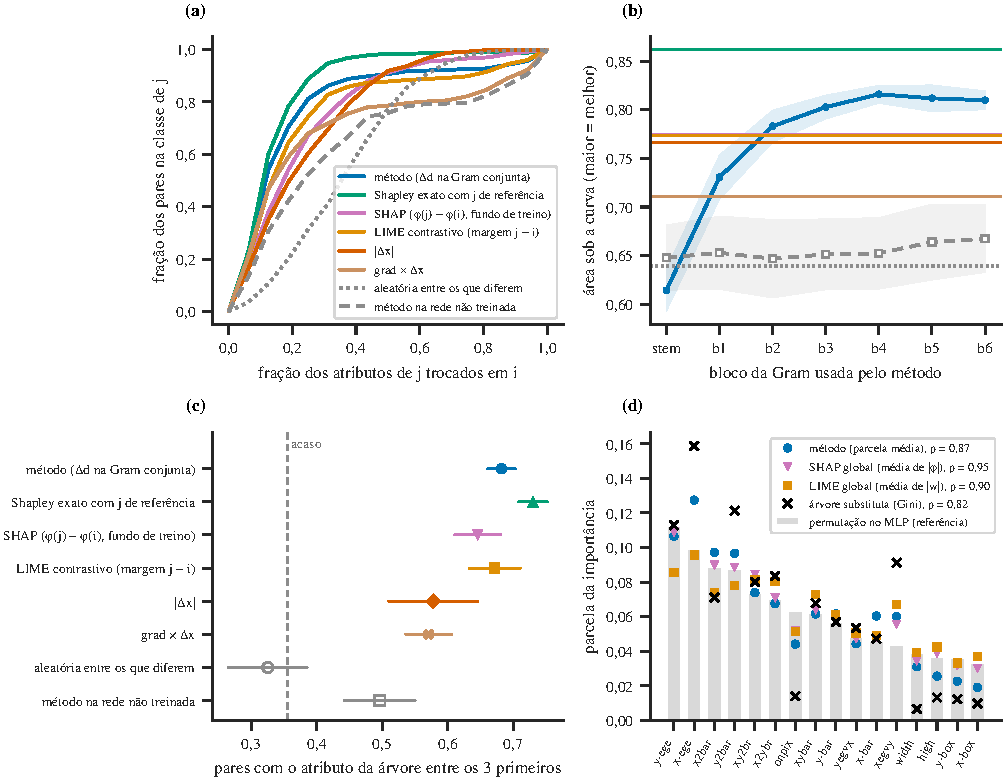
\includegraphics[width=\textwidth]{figuras/res_letter.pdf}
    \caption{Estudo de caso na \texttt{letter}. (a) Curvas de trocas de cada ranking, com o método em \texttt{b3}. (b) Área sob a curva do método em função do bloco, com as referências como linhas horizontais (mesmas cores e estilos de (a)). (c) Fração dos pares em que o atributo de separação da árvore de decisão está entre os três primeiros de cada ranking. (d) Importância global normalizada de cada atributo, na ordem da importância por permutação no perceptron (barras), e a correlação de Spearman de cada fonte com ela.}
    \label{fig:res_letter}
\end{figure}

Três resultados se destacam. O primeiro é que o método supera, em todas as sementes, o SHAP e o LIME nas formas contrastivas ($0{,}803$ contra $0{,}775$ e $0{,}774$) e, com mais folga, nas formas usuais, que explicam apenas a amostra $i$ ($0{,}652$ e $0{,}565$, este último abaixo até da ordem aleatória). A queda é instrutiva: as formas usuais explicam $i$ em relação a uma referência genérica, uma média do treino no SHAP e uma vizinhança amostrada no LIME, e não em relação ao contrafactual $j$. Uma explicação que não é contrastiva não responde à pergunta contrastiva.

O segundo resultado é que o método perde para o valor de Shapley exato com $j$ de referência ($0{,}862$). Isso é esperado, visto que esse jogo é a decomposição exata da própria troca que o teste mede \citep{SundararajanNajmi2020}. Os dois rankings concordam bastante, com correlação de Spearman mediana de $0{,}80$ e o mesmo atributo principal em 78\% dos pares. Uma comparação justa, entretanto, precisa considerar o custo. O método não amostra: ele sempre avalia as $F + 2 = 18$ linhas do par, o que equivale a cerca de 54 avaliações diretas do modelo, enquanto o SHAP e o LIME melhoram com mais avaliações. A Figura \ref{fig:res_orcamento} compara as técnicas com o mesmo orçamento.

\begin{figure}[htbp]
    \centering
    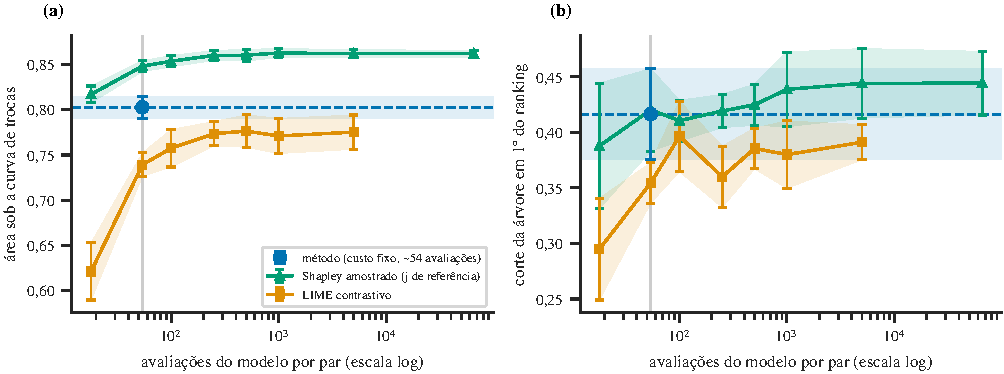
\includegraphics[width=\textwidth]{figuras/res_orcamento.pdf}
    \caption{Comparação com o mesmo orçamento de avaliações do modelo por par, na \texttt{letter} (cinco sementes, cem pares por semente). (a) Área sob a curva de trocas. (b) Fração dos pares em que o atributo de separação da árvore de decisão é o primeiro do ranking. As curvas são o valor de Shapley com $j$ de referência, estimado por permutações amostradas (o último ponto é o valor exato, com $2^{16}$ avaliações), e o LIME contrastivo. O método, que tem custo fixo, é o ponto sobre a linha vertical (cerca de 54 avaliações diretas) e a faixa horizontal. Pontos, barras e faixas indicam a média e o desvio padrão entre as sementes.}
    \label{fig:res_orcamento}
\end{figure}

O resultado divide as duas técnicas. O LIME contrastivo não alcança o método em nenhum orçamento, obtendo $0{,}739 \pm 0{,}013$ com as mesmas 54 avaliações e $0{,}775 \pm 0{,}019$ com cinco mil (Figura \ref{fig:res_orcamento}a). O valor de Shapley com $j$ de referência, ao contrário, supera o método com o mesmo custo, obtendo $0{,}848 \pm 0{,}006$ com três permutações. A explicação é que uma permutação desse jogo é, literalmente, levar os atributos de $i$ ao valor do contrafactual em uma ordem aleatória e registrar a variação da margem, isto é, o próprio teste. Na corroboração pela árvore, entretanto, as duas técnicas empatam com o mesmo custo (Figura \ref{fig:res_orcamento}b). A vantagem do método, portanto, não está no teste de trocas em si, e sim em que a mesma geometria responde também às perguntas P1 a P5, fornece a leitura por bloco e, como mostra a Subseção \ref{subsec:res_arquitetura}, recupera a explicação de uma árvore de decisão melhor do que o próprio Shapley exato.

O terceiro resultado é a corroboração por um modelo independente. A árvore de decisão treinada sobre os rótulos atinge acurácia de $0{,}850$ e concorda com o perceptron em 85\% das amostras de teste. Nos pares em que ela reproduz as duas predições, o atributo em que ela separa $i$ de $j$ está entre os três primeiros do método em 69\% dos pares, contra 68\% do LIME contrastivo, 66\% do SHAP e 36\% do acaso (Figura \ref{fig:res_letter}c). Isto é, dois modelos de natureza diferente apoiam-se nos mesmos atributos para distinguir as mesmas amostras, e o método recupera esse acordo a partir da geometria interna da rede. A árvore, entretanto, precisa de cerca de 1\,200 folhas e profundidade 27 para alcançar essa acurácia, o que a torna pouco legível e reforça o argumento de explicar o modelo que se usa, e não um substituto mais simples \citep{Rudin2019}.

Por fim, o método mostra em que profundidade da rede cada atributo passa a importar, algo que o SHAP e o LIME não separam. Em um par em que o perceptron classifica uma letra como G e outra como E, a dispersão horizontal dos píxeis acesos (\texttt{x2bar}) responde por 0\% da aproximação no \texttt{stem}, por 36\% em \texttt{b3} e novamente por 0\% em \texttt{b6}, isto é, essa distinção é usada no meio da rede e depois absorvida. No nível global, por outro lado, o SHAP ($0{,}95$) e o LIME ($0{,}90$) concordam mais com a importância por permutação do que o método ($0{,}87$) e a árvore ($0{,}82$) (Figura \ref{fig:res_letter}d).

\subsubsection*{Nas imagens}

Nas imagens, a leitura usa a Gram cruzada de duas imagens. Sobre vinte pares do Pet, entre raças que o modelo confunde ou da mesma raça com uma classificação correta e outra errada, o mapa do método derruba a margem $f_{c_i} - f_{c_j}$ mais do que a rede não treinada e a ordem aleatória, mas não supera o mapa de centro e falha no piso de especificidade: o mesmo mapa calculado contra uma terceira imagem, de raça não envolvida, derruba a margem quase tanto. O Grad-CAM contrastivo, calculado sobre o gradiente da mesma margem, supera o método a partir de \texttt{b4}. Sendo assim, nas imagens, o mapa indica quais regiões sustentam a decisão de $i$, e não quais a distinguem do contrafactual $j$.

\subsection{P7: As leituras dependem do modelo?}\label{subsec:res_arquitetura}

Esta pergunta é respondida em dois níveis: o mesmo código aplicado a um transformador de visão e o método aplicado a um modelo que não é uma rede neural, a árvore de decisão da \texttt{letter}.

\subsubsection*{O transformador de visão}

\begin{table}[htbp]
\centering
\caption{Leituras por imagem no Oxford-IIIT Pet para as duas arquiteturas (três sementes cada, alvo fixo), do \texttt{stem} a \texttt{b6}, e o piso cruzado de cada uma. Todas as leituras superam o piso em todas as sementes a partir de \texttt{b1}, exceto $\widehat{E}_{\mathrm{ratio}}$ nos blocos rasos da ResNet.}
\label{tab:res_arquitetura}
\small
\begin{tabular}{l c c c c}
\hline
 & \multicolumn{2}{c}{ResNet} & \multicolumn{2}{c}{Transformador} \\
Leitura & Conjunta & Piso & Conjunta & Piso \\
\hline
$k$-vizinhos contra a predição & $0{,}069 \to 0{,}603$ & $0{,}06$ & $0{,}132 \to 0{,}559$ & $0{,}04$ a $0{,}07$ \\
AUC da margem para o acerto & $0{,}591 \to 0{,}865$ & $0{,}54$ a $0{,}56$ & $0{,}629 \to 0{,}823$ & $0{,}51$ a $0{,}52$ \\
Confusão suave (Spearman) & $0{,}170 \to 0{,}674$ & $0{,}21$ & $0{,}495 \to 0{,}738$ & $0{,}09$ a $0{,}24$ \\
Contenção em $V_r$ ($r = K-1$) & $0{,}112 \to 0{,}325$ & $0{,}10$ & $0{,}139 \to 0{,}240$ & $0{,}10$ \\
$\widehat{E}_{\mathrm{ratio}}$ para o erro & $0{,}485 \to 0{,}615$ & $0{,}53$ a $0{,}55$ & $0{,}507 \to 0{,}663$ & $0{,}52$ a $0{,}54$ \\
\hline
\end{tabular}
\end{table}

As leituras por imagem se transferem ao transformador sem nenhuma alteração do código (Tabela \ref{tab:res_arquitetura}), e a razão de energia ortogonal, que falhava nos blocos rasos da ResNet, supera o piso em todas as sementes de \texttt{b1} a \texttt{b6}. O que muda é a origem da informação. No transformador, o gradiente contrastivo isolado quase não carrega informação sobre o comportamento, e a composição só supera as ativações de forma consistente no \texttt{stem}, de modo que a decomposição contra a CKA favorece a CKA a partir de \texttt{b2}. A contenção em $V_r$, por outro lado, continua favorecendo a composição em todos os blocos. Sendo assim, a forma do método independe da arquitetura, mas a contribuição de cada fonte não: o que o gradiente acrescenta às ativações é uma propriedade da rede convolucional, e não do método.

\begin{figure}[htbp]
    \centering
    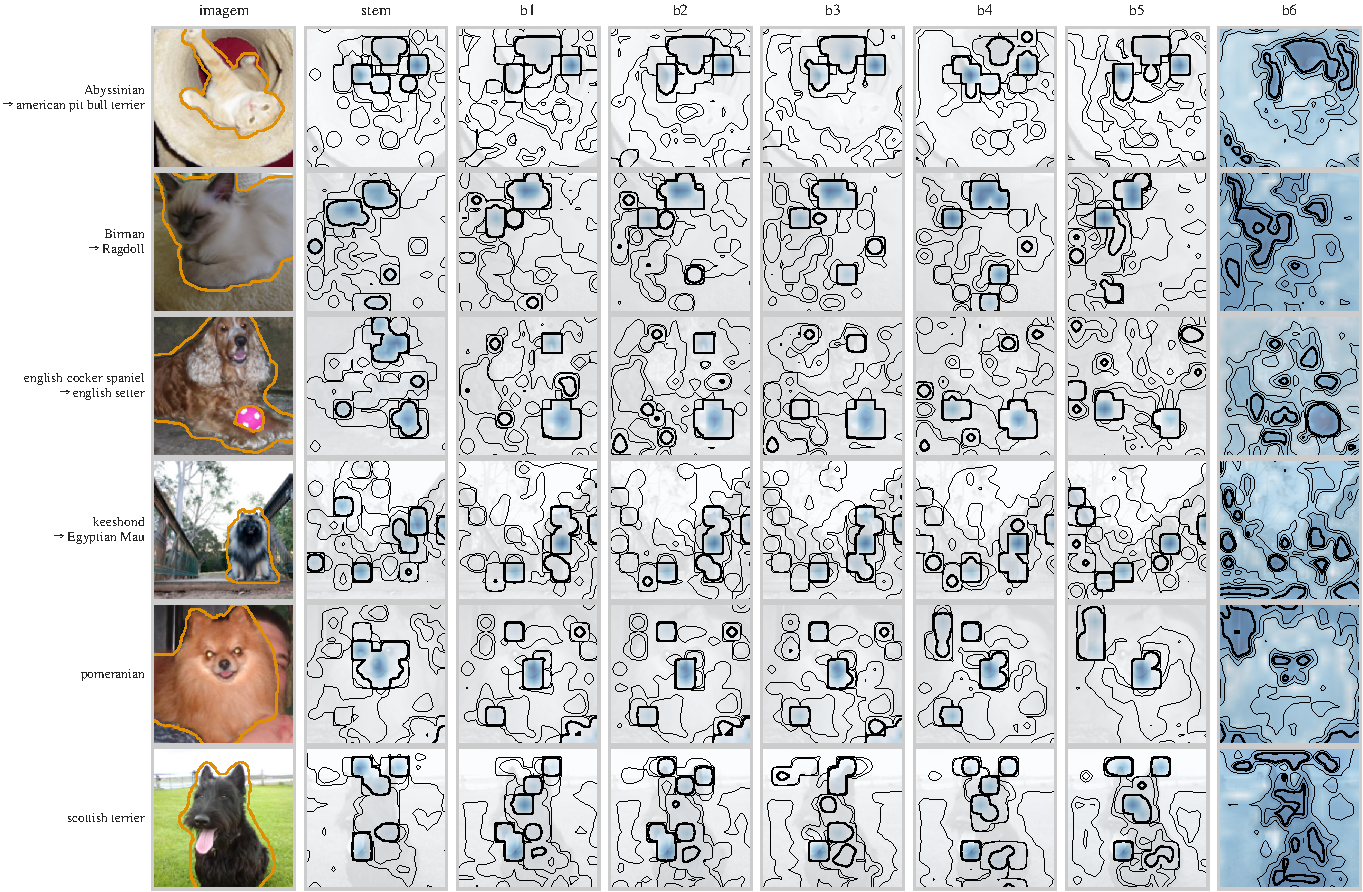
\includegraphics[width=\textwidth]{figuras/res_campo_vit.pdf}
    \caption{Campo de energia da Gram conjunta do transformador sobre as mesmas imagens da Figura \ref{fig:res_campo_resnet}. O aspecto quadriculado vem da grade de \textit{tokens} ($16 \times 16$), ampliada para a imagem. No último bloco, a cabeça é um \textit{pooling} médio seguido de uma camada linear, de modo que o gradiente é o mesmo em todas as posições e o campo deixa de distinguir regiões.}
    \label{fig:res_campo_vit}
\end{figure}

As leituras sobre a entrada, entretanto, não se transferem. No transformador, a fração da energia sobre o animal cai de $0{,}83$ no \texttt{stem} para perto do piso de centro nos blocos seguintes, e o teste de deleção fica abaixo do centro em todos os blocos (Figura \ref{fig:res_campo_vit}). A explicação mais provável é estrutural: a atenção mistura informação de toda a imagem já nas primeiras camadas \citep{Raghu2021}, e o vetor de um \textit{token} deixa de descrever apenas a sua posição. Por esse motivo, as leituras espaciais em transformadores costumam propagar a relevância através da atenção \citep{Chefer2021}. Essa explicação, contudo, não foi separada da baixa acurácia do modelo.

\subsubsection*{O método aplicado a uma árvore de decisão}

O segundo nível testa se o método é, de fato, modelo-agnóstico. A árvore de decisão da \texttt{letter} é analisada com as fontes de caminho, folga e classes, com a mesma composição e a mesma leitura de pares utilizadas nas redes, e as suas leituras são comparadas com uma resposta conhecida, a explicação que a própria árvore fornece pelo seu caminho de decisão.

A Figura \ref{fig:res_arvore_caminhos} mostra, para dois pares, essa explicação e a leitura do método lado a lado. O método não tem acesso à regra de decisão da árvore: ele apenas compõe as três fontes e mede quanto levar cada atributo ao valor do contrafactual aproxima $i$ de $j$. Ainda assim, o atributo testado no nó de separação passa a responder por praticamente toda a pontuação exatamente na profundidade em que os caminhos se separam. Nas profundidades anteriores, os dois caminhos são idênticos, e a única fonte que distingue as amostras é a folga, isto é, o quanto cada uma está distante dos limiares que ambas atravessaram.

\begin{figure}[htbp]
    \centering
    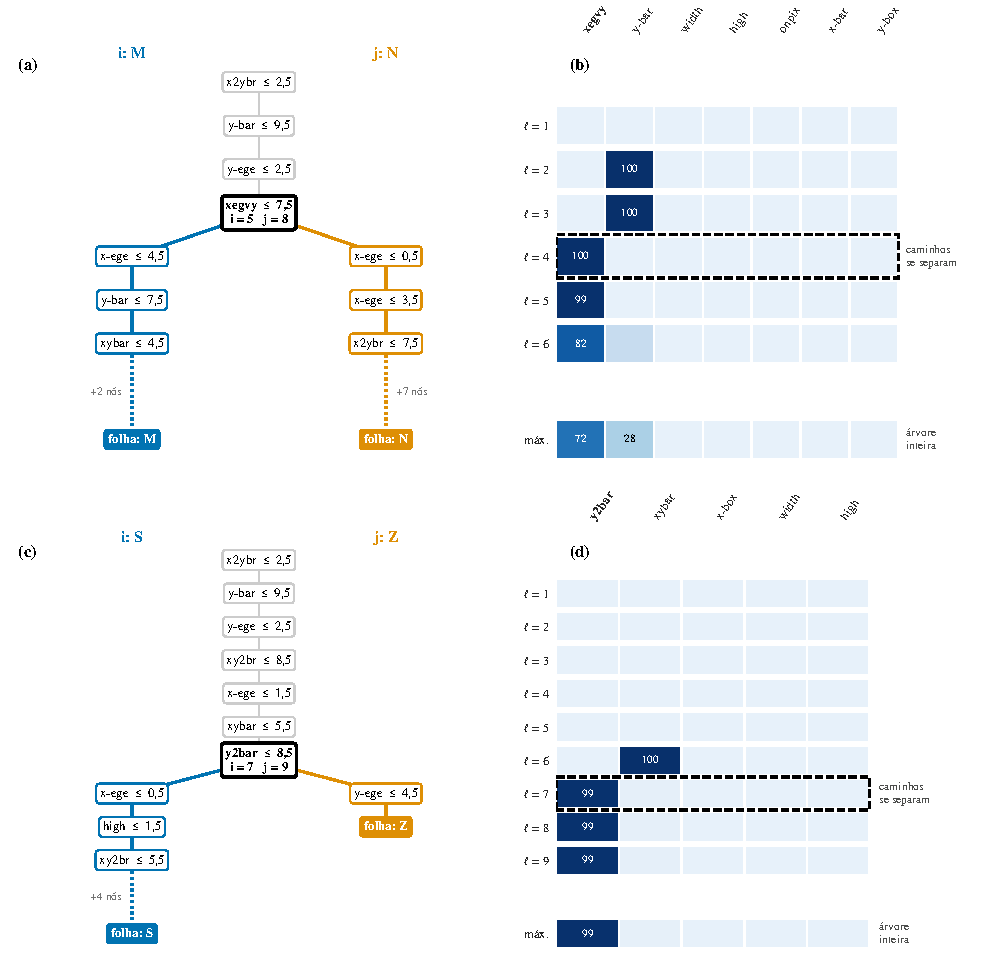
\includegraphics[width=\textwidth]{figuras/res_arvore_caminhos.pdf}
    \caption{A explicação da árvore de decisão e a leitura do método, lado a lado, para dois pares da \texttt{letter} (semente 0). (a, c) Caminhos das amostras $i$ (azul) e $j$ (laranja) na árvore: o trecho comum, o nó de separação (destacado, com os valores de $i$ e de $j$ no atributo testado) e os ramos até as folhas, com os nós intermediários omitidos. (b, d) Parcela de cada atributo, em porcentagem, na pontuação $\Delta d_f$ do método em cada profundidade $\ell$, alinhada verticalmente com a árvore. A linha tracejada marca a profundidade em que os caminhos se separam, e a última linha é a árvore inteira. As colunas são os atributos que diferem entre $i$ e $j$, na ordem do ranking final do método, e o atributo de separação está em negrito. Os dois pares ilustram o caso típico, em que a datação do método coincide com a da árvore (81\% dos pares).}
    \label{fig:res_arvore_caminhos}
\end{figure}

\begin{table}[htbp]
\centering
\caption{O método aplicado a uma árvore de decisão na \texttt{letter} (cinco sementes, cem pares por semente). Fração dos pares em que o atributo do nó em que os caminhos de $i$ e $j$ se separam é o primeiro de cada ranking, e área sob a curva do teste de trocas feito na própria árvore.}
\label{tab:res_arvore}
\small
\begin{tabular}{l c c}
\hline
Ranking & Corte da árvore em 1º & Área de trocas na árvore \\
\hline
\textbf{Método} (caminho $\circ$ folga $\circ$ classes) & $\mathbf{0{,}856}$ & $\mathbf{0{,}630}$ \\
Só caminho & $0{,}984$ & $0{,}628$ \\
Só folga & $0{,}852$ & $0{,}594$ \\
Só classes & $0{,}478$ & $0{,}603$ \\
Shapley exato com $j$ de referência & $0{,}766$ & $0{,}901$ \\
$|\Delta x|$ & $0{,}234$ & $0{,}716$ \\
Aleatória entre os que diferem & $0{,}132$ & $0{,}663$ \\
Método na árvore de rótulos embaralhados & $0{,}124$ & $0{,}466$ \\
\hline
\end{tabular}
\end{table}

\begin{figure}[htbp]
    \centering
    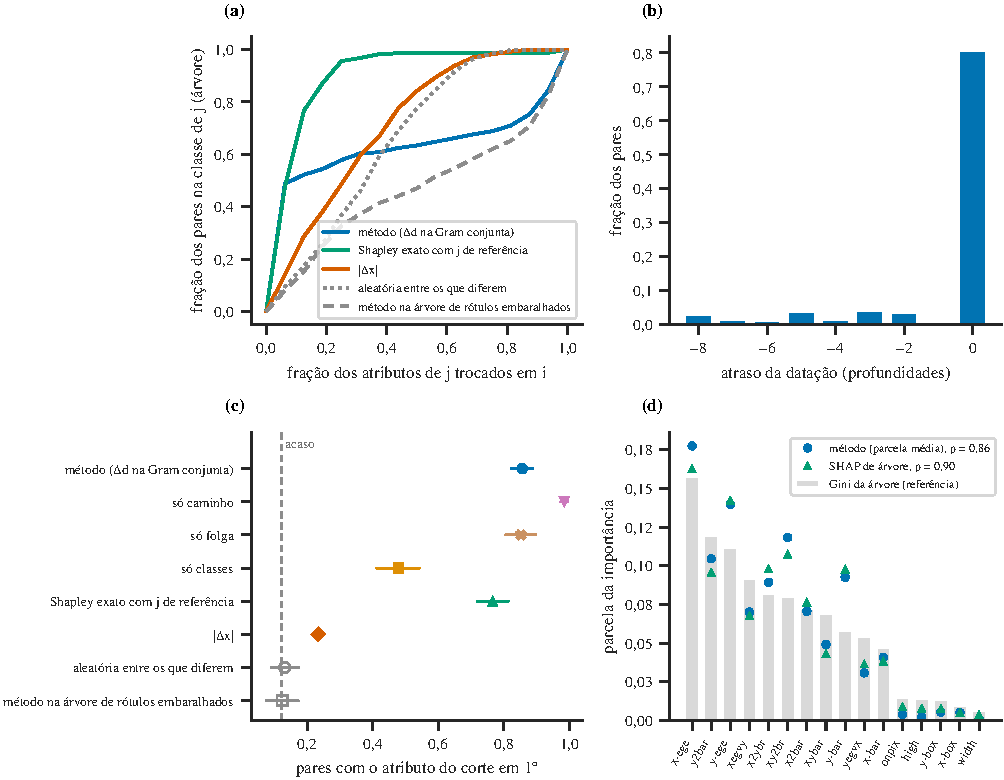
\includegraphics[width=\textwidth]{figuras/res_arvore.pdf}
    \caption{O método aplicado a uma árvore de decisão na \texttt{letter}. (a) Teste de trocas na própria árvore. (b) Diferença entre a profundidade em que o atributo de separação passa a ser o primeiro do método e a profundidade em que os caminhos de $i$ e $j$ se separam. (c) Fração dos pares em que o atributo de separação é o primeiro de cada ranking. (d) Importância global normalizada, na ordem da importância de Gini da árvore.}
    \label{fig:res_arvore}
\end{figure}

Em termos agregados (Tabela \ref{tab:res_arvore}), o atributo do nó de separação é o primeiro do método em 86\% dos pares, contra 77\% do Shapley exato, 23\% da diferença bruta e 12\% do piso. A fonte de caminho sozinha alcança 98\%, o que é quase uma consequência da construção, visto que trocar esse atributo é o que muda o caminho de $i$. O resultado não trivial é a datação: a profundidade em que o atributo de separação passa a ser o primeiro do método coincide com a profundidade da separação em 81\% dos pares e nunca ocorre depois dela (Figura \ref{fig:res_arvore}b). Nos demais pares, ela ocorre antes, quase sempre porque um nó acima da separação testa o mesmo atributo e a folga registra essa proximidade de um limiar. No nível global, a parcela média do método tem correlação de $0{,}86$ com a importância de Gini e de $0{,}94$ com o SHAP de árvore \citep{Lundberg2020}.

O mesmo experimento expõe o principal limite da leitura de pares. No teste de trocas na própria árvore, o método obtém $0{,}630$, abaixo da diferença bruta ($0{,}716$), e precisa, em média, de $5{,}8$ trocas para produzir um contrafactual válido, contra $1{,}7$ do contrafactual mínimo, obtido por enumeração. A causa é que $\Delta d_f$ troca um atributo de cada vez: os atributos que só importam depois que $i$ atravessa o corte não alteram nada quando trocados sozinhos, e ficam em ordem arbitrária no ranking. O valor de Shapley, que considera todas as combinações de trocas, enxerga essas interações. Sendo assim, a leitura de pares responde o que distingue $i$ do seu contrafactual, e não o menor conjunto de mudanças que basta para que $i$ se torne $j$.

\subsection{P8: Em que profundidade a decisão se forma?}\label{subsec:res_datacao}

A intervenção da Equação \eqref{eq:intervencao} fornece uma datação externa ao método: depois que a decisão está formada, o estado passa a ser redundante com ela e se torna robusto a perturbações. A correlação de Spearman entre essa estabilidade e a recuperação da decisão pela Gram conjunta é positiva em todas as bases tabulares, de $0{,}87 \pm 0{,}11$ na ResNet e de $1{,}00$ no transformador.

Essa concordância, entretanto, é mais fraca do que aparenta, pois as duas séries são monótonas na profundidade, e o valor observado decorre em boa medida dessa monotonicidade comum. O mesmo problema é conhecido nas sondagens lineares, em que a capacidade de decodificar uma propriedade cresce com a profundidade sem indicar onde o modelo a utiliza \citep{Belinkov2022}. Nas redes, a afirmação sustentada é apenas que as duas datações não se contradizem. A verificação genuína vem da árvore de decisão, em que a profundidade da decisão é conhecida para cada par e o método a acerta exatamente em 81\% dos pares.

\subsection{Custo computacional medido}\label{subsec:res_custo}

A análise da Subseção \ref{subsec:custo} foi verificada medindo o tempo de cada etapa enquanto o tamanho do problema cresce. Em escala logarítmica, um custo $\Theta(n^a)$ aparece como uma reta de inclinação $a$, e é essa inclinação que a Figura \ref{fig:res_complexidade} reporta.

\begin{figure}[htbp]
    \centering
    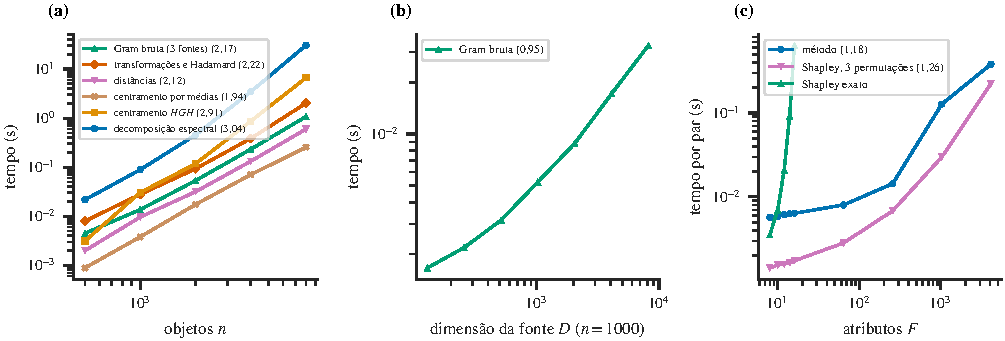
\includegraphics[width=\textwidth]{figuras/res_complexidade.pdf}
    \caption{Tempo das etapas do método em função do tamanho do problema, em escala logarítmica nos dois eixos. Entre parênteses está a inclinação ajustada nos três maiores tamanhos, que estima o expoente do custo. (a) Etapas da construção e das leituras em função do número de objetos $n$, com três fontes de dimensão 256. (b) Matriz de Gram bruta em função da dimensão $D$ da fonte, com $n = 1\,000$. (c) Leitura de diferenças entre pares em função do número de atributos $F$, comparada ao valor de Shapley exato com $j$ de referência e à sua estimativa por três permutações.}
    \label{fig:res_complexidade}
\end{figure}

Os expoentes medidos coincidem com os previstos. A matriz de Gram bruta cresce como $\Theta(n^2 D)$ (expoentes $2{,}17$ em $n$ e $0{,}95$ em $D$), as transformações, o produto de Hadamard e a matriz de distâncias crescem com expoente próximo de 2 e a decomposição espectral com $3{,}04$. As alternativas quadráticas da Tabela \ref{tab:custo} também se confirmam: o centramento pelas médias de linhas e colunas leva $0{,}25$ s com $n = 8\,000$, contra $6{,}6$ s do produto $H\widetilde{\mathbf{G}}H$. Com $n \approx 500$, entretanto, a decomposição leva cerca de $22$ ms, e o custo total é dominado pela extração das fontes. A leitura de pares confirma o custo linear no número de atributos (Figura \ref{fig:res_complexidade}c), enquanto o valor de Shapley exato dobra a cada atributo acrescentado. A sua estimativa por permutações, entretanto, também é linear e, por utilizar apenas passagens diretas, é mais rápida que o método por par.
